\documentclass[11pt]{article}

\usepackage{url,amsmath,amsfonts,amssymb, bm}
\usepackage{amssymb}
\usepackage{graphicx}
\usepackage{enumerate}
\usepackage{url,amsmath,amsfonts,amssymb, bm}
\usepackage{subfig}
\usepackage{caption}
%\usepackage{multirow}

\newtheorem{definition}{Definition}
\newtheorem{remark}{Remark}
\newtheorem{properties}{Properties}
\newtheorem{example}{Example}
\newtheorem{theorem}{Theorem}
\newtheorem{lemma}[theorem]{Lemma}
\newtheorem{corollary}[theorem]{Corollary}
\newtheorem{proposition}[theorem]{Proposition}
\newtheorem{claim}[theorem]{Claim}
\newtheorem{observation}{Observation}

\def \endprf{\hfill {\vrule height6pt width6pt depth0pt}\medskip}
\newenvironment{proof}{\noindent {\bf Proof} }{\endprf\par}

\newcommand{\R}{{\mathbb R}}
\newcommand{\Z}{{\mathbb Z}}
\newcommand{\Q}{{\mathbb Q}}
\newcommand{\C}{{\mathbb C}}
\newcommand{\N}{{\mathbb N}}


\newcommand{\E}{{\mathbb E}}

\newcommand{\A}{\mathcal{A}}

\newlength{\toppush}
\setlength{\toppush}{2\headheight}
\addtolength{\toppush}{\headsep}

\newcommand{\htitle}[4]{\noindent\vspace*{-\toppush}\newline\parbox{6.5in}
{\begin{center} {\bf HOMEWORK \#4}\end{center}
\begin{center} {University of Southern California}\end{center}
#1  \hfill  
 #3 \hfill #4 \newline
\mbox{}\hrulefill\mbox{}}\vspace*{1ex}\mbox{}\newline
\begin{center}{\Large\bf #2}\end{center}}

\newcommand{\handout}[3]{\thispagestyle{empty}
 \markboth{ #2}{ #2}
 \pagestyle{myheadings}\htitle{\protect\ref{#1}}{#2}{#3}}

\setlength{\oddsidemargin}{0pt}
\setlength{\evensidemargin}{0pt}
\setlength{\textwidth}{6.5in}
\setlength{\topmargin}{0in}
\setlength{\textheight}{8.5in}

\newcommand{\vct}[1]{\bm{#1}}
\newcommand{\mtx}[1]{\bm{#1}}

\begin{document}

%%%%% Fill in the lecture number, date, and your name here.
\htitle{Lecturer: C.-C.JayKuo}{Report}{Issued: 3/4/2019}{Due:3/19/2019}


\section{Problem 1: Texture Analysis}
\subsection{Texture Classification}
\subsubsection{Abstract and Motivation}
Texture is a description of the spatial arrangement of color or intensities in an image or a selected region of an image. Laws developed a series of filters that could automatically detect the texture patterns. Laws' masks are well established as one of the best methods for texture analysis in image processing and are used in various applications, including medical image analysis. In this section, I use the five 1D laws filters to extract the features of 12 textures images and use kmeans method to classification.\par
\subsubsection{Approach and Procedures}

\begin{enumerate}
\item Preprocessing\\
First of all, extend the image boundary with 2 pixels width for each edge by reflection. Then, normalize the input image pixel value by,
\begin{equation}
I(i,j)= \frac { I(i,j) }{ 255 } 
\end{equation}
Use the result image as the input for the following steps.\par

\item Set up the Laws filter \\
The 2D Laws' filter is caculated by using 1D filter. The five 1D filters are as follows.
\begin{equation}
\begin{aligned}
L5&=[1,4,6,4,1]\\
E5&=[-1,-2,0,2,1]\\
S5&=[-1,0,2,0,-1]\\
W5&=[-1,2,0,-2,1]\\
R5&=[ 1,-4,6,-4,1]
\end{aligned}
\end{equation}
This filter detect level, edge, spot, wave and ripple of the input image.
The 2D Laws' filter is the outer product of the 1D laws filters. Thus, we can finally get 25 2D Laws' filters. For one Laws filter, it detect the different property in different direction. Take the E5S5 as an example, the E5S5 is  
\begin{equation}
E5S5=\begin{bmatrix} 1 & 0 & -2 & 0 & 1 \\ 2 & 0 & -4 & 0 & 2 \\ 0 & 0 & 0 & 0 & 0 \\ -2 & 0 & 4 & 0 & -2 \\ -1 & 0 & 2 & 0 & -1 \end{bmatrix}
\end{equation}
In the vertical direction, it detect the edge characteristic of the image, while in the horizontal direction, it detect the spot characteristic.\par
\item Convolution and Caculate the Energy\\
Use the 2D filter obtained above, convolute the input image and get a filtered image. Caculate the square sum as the representation of the energy using the following equation,

\begin{equation}
Square\_ sum=\sqrt { \frac { 1 }{ MN } \sum _{ i=1 }^{ i=M }{ \sum _{ j=1 }^{ j=N }{ { I(i,j) }^{ 2 } }  }  } 
\end{equation}
Where, $M$ is the height and $N$ is the width of the image. The $Square\_ sum$ is represent the texture property obtained by each filter. After filtered with 25 2-D laws filters, we can finally get a 1 by 25 dimension vector for each images. Since we have 12 texture images, we finally get a $12 \times 25$ two-dimension array.\par
\item Principal Component Analysis \\
Suppose the input matix is a $N \times D$ matrix, where each row represent a training point while each column represent the feature of the data.\par
First, normalize the feature of each data into zero mean and unit variance, i.e. subtract the mean from each column and divided its variance. 
\begin{equation}
X(:,i)=\frac { X(:,i)-\mu  }{ var } 
\end{equation}
\par
Second, caculate the covariance matrix ${\mtx C}$.
\begin{equation}
cov(\mtx C)=\mtx X^{ T }\mtx X
\end{equation}
\par
Third, do the SVD decomposition of ${\mtx C}$.
\begin{equation}
\mtx C=\mtx U \mtx \Sigma \mtx V^{ T } = \sum _{ i=1 }^{ i=D }{ u_{i}\sigma_{i}v_{i} } 
\end{equation}
Where $\sigma_{1}, \sigma_{2} ... \sigma_{D}$ is the sigular value sorted in decreasing order. Pick the first three largest sigular value and the corresponding left and right singular vectors to form the new low dimension dataset.
\par
Last, recover the low-dimension data by multiply the first three columns of the left-sigular-vector ${\mtx U(:,1:3)}$.
\begin{equation}
\hat { \mtx X } =\mtx X\times \mtx U(:,1:3)
\end{equation}

\item K-means Clustering\\
For a dataset ${\vct x_1,...,\vct x_N} \in \mathbb{R}^D $, the K-means distortion objective function is, 
\begin{equation}
J(\{ \mu _{ k }\} ,\{ r_{ ik }\} )=\frac { 1 }{ N } \sum _{ i=i }^{ N }{ \sum _{ k=1 }^{ K }{ r_{ ik }\parallel { \mu  }_{ k }-{\vct x }_{ i }\parallel_{2} ^{ 2 } }  } 
\end{equation}

Where ${ \mu_1,...,\mu_N}$ are the centroids of K clusters and $r_{ik} \in \{0,1\}$ represent whether example $i$ belongs to cluster $k$. Our goal is to minimize $J$ by update the centroid and clusters over iteration. \par
First, fixing the centroid and cluster the dataset. The cluster clasification is measured by Euclidean distance.
\begin{equation}
\hat { r_{ ik } } =\begin{cases} 1\quad k=argmin_{ k' }\left\| \mu _{ k' }-\vct x_{ i } \right\| ^{ 2 }_{ 2 } \\ 0\quad else \end{cases}
\end{equation}
Second, fixing the cluster assignment and find the new centroid by minimize $J$. 
\begin{equation}
\hat { { \mu  }_{ k } } =\frac { \sum _{ i=1 }^{ N }{ { r }_{ ik }{\vct x }_{ i } }  }{ \sum _{ i=1 }^{ N }{ { r }_{ ik } }  } 
\end{equation}
By repeating this two steps, k-means finally cluster the input data into k cluster until the maximum iteration is reached.
\end{enumerate} 
\subsubsection{Experimental Result}
The feature obtained by laws filters are shown in Table \ref{laws}.

\begin{table}[!htp]
\caption{Laws' filter Results}
\resizebox*{170mm}{21mm}{
\begin{tabular}{llllllllllllllllllllllllll}
\hline
           & L5L5             & L5E5             & L5S5             & L5W5             & L5R5             & E5L5             & E5E5              & E5S5              & E5W5              & E5R5              & S5L5              & S5E5              & S5S5              & S5W5              & S5R5              & W5L5              & W5E5              & W5S5              & W5W5              & W5R5              & R5L5             & R5E5              & R5S5              & R5W5              & R5R5              \\ \hline
Texture 1  & 23.234247 & 4.6825110 & 2.1976640 & 1.8063850 & 2.8931140 & 4.6563900 & 1.14569  & 0.615261 & 0.543338 & 0.911480 & 2.2360650  & 0.629166 & 0.366846 & 0.340821 & 0.596002 & 1.8570570  & 0.571519 & 0.353790 & 0.344430 & 0.624239 & 3.0070380 & 0.992611 & 0.650907 & 0.669362 & 1.2684020  \\
Texture 2  & 15.519040 & 3.3037110 & 2.0008330 & 1.9259510 & 3.3339640 & 3.0939180 & 1.0554210  & 0.705943 & 0.718552 & 1.3054350  & 1.9633920  & 0.664501 & 0.458605 & 0.483221 & 0.948022 & 1.8790030  & 0.650536 & 0.465297 & 0.504723 & 1.0278850  & 4.22519 & 1.2137740  & 0.912609 & 1.0329280  & 2.1175560  \\
Texture 3  & 16.621194 & 4.4736080 & 3.31508 & 3.6534520 & 7.0009330 & 1.6925420 & 0.360978 & 0.227988 & 0.234451 & 0.474318 & 1.1261190  & 0.206598 & 0.133033 & 0.137970 & 0.279465 & 1.0865340  & 0.203801 & 0.133234 & 0.140679 & 0.289675 & 3.1793560 & 0.408892 & 0.270087 & 0.291381 & 0.608785 \\
Texture 4  & 23.468594 & 6.7505890 & 3.9780370 & 3.6511910 & 6.1144190 & 4.7540730 & 1.4080920  & 0.869330 & 0.840918 & 1.52497  & 2.6181890  & 0.774082 & 0.483874 & 0.472601 & 0.875657 & 2.4161390  & 0.724981 & 0.458069 & 0.452810 & 0.844226 & 4.9179660 & 1.3020250  & 0.836251 & 0.843531 & 1.6102970  \\
Texture 5  & 42.057818 & 9.6580320 & 4.8892210 & 3.9949350 & 6.3130140 & 9.2229180 & 2.4742920  & 1.3526740  & 1.1989280  & 2.0053660  & 4.7171120  & 1.3507530  & 0.791898 & 0.737567 & 1.2900120  & 4.00038  & 1.2359560  & 0.764760 & 0.742231 & 1.3488630  & 7.1464640 & 2.2008030  & 1.4254330  & 1.4459380  & 2.7398020  \\
Texture 6  & 37.257672 & 10.672662 & 6.2258550 & 5.6340540 & 9.3717850 & 7.3090420 & 2.2058610  & 1.3637470  & 1.3177120  & 2.4033310  & 3.8956840  & 1.2125590  & 0.763727 & 0.750567 & 1.4043120  & 3.5644950  & 1.1379410  & 0.725143 & 0.722346 & 1.3721710  & 6.62047 & 2.0481660  & 1.3286520  & 1.3556710  & 2.6589960  \\
Texture 7  & 22.204380 & 5.1025030 & 2.5982240 & 2.1287460 & 3.3601380 & 4.8471780 & 1.3032860  & 0.717721 & 0.637370 & 1.0668270  & 2.5244110  & 0.712157 & 0.419269 & 0.390548 & 0.683647 & 2.1683510  & 0.653331 & 0.405365 & 0.393021 & 0.713837 & 4.1362860 & 1.1646540  & 0.756777 & 0.767413 & 1.44918  \\
Texture 8  & 29.347879 & 6.2740220 & 3.7880610 & 3.6377180 & 6.3145750 & 5.7985960 & 2.0565240  & 1.3701370  & 1.3871990  & 2.5091330  & 3.4533610  & 1.3089360  & 0.905245 & 0.949446 & 1.8488910  & 3.2782250  & 1.2890810  & 0.929327 & 1.00544  & 2.0269070  & 6.2573210 & 2.3843810  & 1.8114760  & 2.0633110  & 4.2256870  \\
Texture 9  & 43.238528 & 9.1141560 & 6.7507420 & 7.3943790 & 13.912112 & 3.7394160 & 0.900478 & 0.563597 & 0.582703 & 1.1947090  & 1.9297210  & 0.524479 & 0.339574 & 0.355980 & 0.739276 & 1.9029960  & 0.536469 & 0.353914 & 0.375567 & 0.789401 & 4.2254170 & 1.0991890  & 0.736089 & 0.796160 & 1.6858160  \\
Texture 10 & 23.015021 & 4.8983070 & 3.2974780 & 3.42569 & 6.6216140 & 2.3702640 & 0.976126 & 0.759602 & 0.889031 & 1.9975260  & 1.0646410  & 0.428021 & 0.343537 & 0.423066 & 1.0391950  & 0.890206 & 0.327091 & 0.256623 & 0.319995 & 0.834625 & 1.4483590 & 0.505643 & 0.387378 & 0.4711 & 1.2521780  \\
Texture 11 & 16.264758 & 4.8344790 & 3.1763660 & 3.0221690 & 4.5084640 & 1.3376630 & 0.332087 & 0.217935 & 0.234377 & 0.495369 & 0.779485 & 0.188805 & 0.125442 & 0.137253 & 0.300436 & 0.780822 & 0.187067 & 0.126896 & 0.1405 & 0.310427 & 1.5282950 & 0.379609 & 0.260953 & 0.293954 & 0.662665 \\
Texture 12 & 26.865751 & 6.6678070 & 3.6361530 & 3.2245420 & 5.4255880 & 4.5457440 & 1.38110  & 0.773449 & 0.740840 & 1.3593010  & 2.3570780  & 0.697736 & 0.423219 & 0.415515 & 0.790853 & 2.1023390  & 0.640086 & 0.395435 & 0.395456 & 0.766898 & 3.55898 & 1.1281490  & 0.721796 & 0.744824 & 1.4777550  \\ \cline{1-26} 
\end{tabular}}
\label{laws}
\end{table}

The plot of PCA is shown in Figure \ref{pca_3d}.
\begin{figure}[!htp]
	\centering
	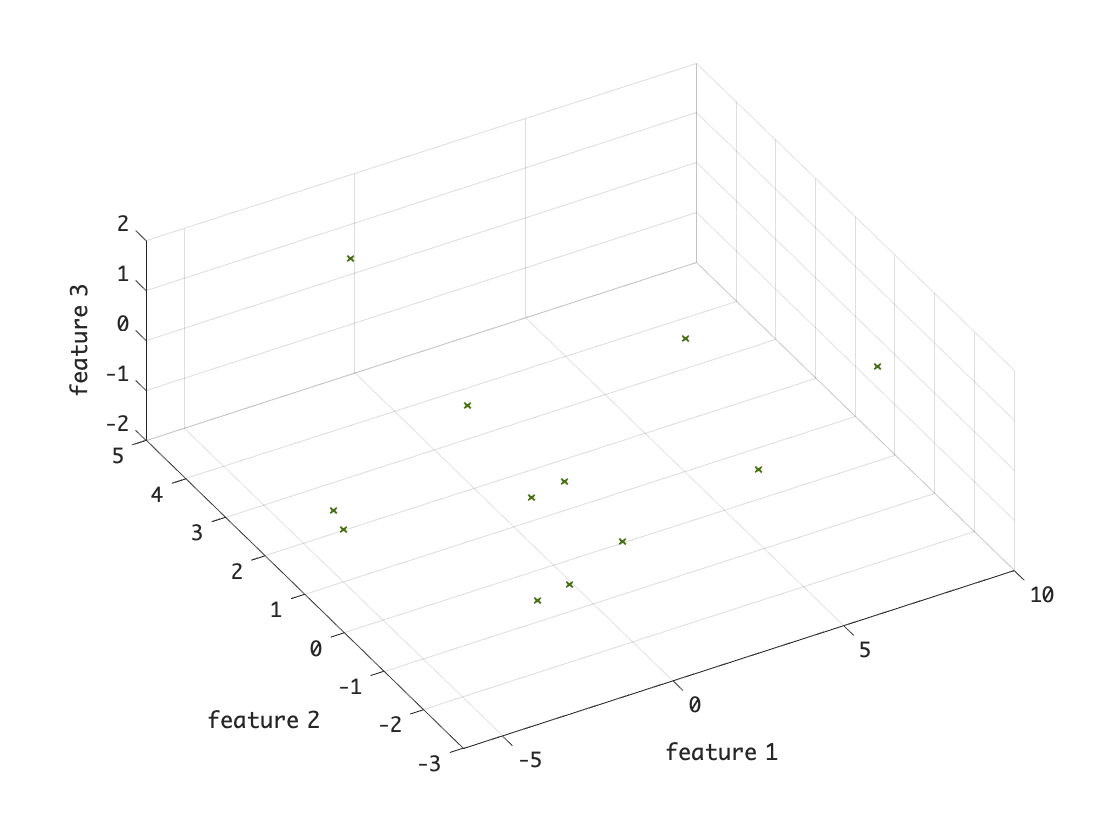
\includegraphics[scale=0.3]{pca_3d.png}
	\caption{PCA Result}
	\label{pca_3d}
	\end{figure}
\par
The kmeans result are as follows.\par

Groud truth: Bark: 4, 6, 12. Straw: 2, 8, 10. Brick: 3, 9, 11. Bubble: 1, 5, 7.\par
Use 25 dimension feature space to do the kmeans: 1, 2, 3, 1, 4, 4, 1, 1, 4, 1, 3, 1.\par
Use 3 dimension feature space to do the kmeans: 2, 2, 3, 1, 4, 4, 2, 4, 1, 2, 3, 1. \par
\subsubsection{Discussion}

Compute the variance of each feature over 12 images, we can conclude that L5L5 maintains the largest discriminant power, that could distingush each images. That is because the L5L5 filter collects the low-dimension information of the input image, which is dominant in the image. Beside, the Numerical value is the highest among the features. Thus, a small fluctuation of L5L5 will result in a large variance in the feature space. On the other hand, S5W5 maintains the smallest discriminant power, because S5E5 extract the high frequency information which is of small quantity in the images. \par
\begin{table}[!htp]
\centering
\caption{Variance of the 25-D features}
\resizebox*{170mm}{5mm}{
\begin{tabular}{|l|l|l|l|l|l|l|l|l|l|l|l|l|l|l|l|l|l|l|l|l|l|l|l|l|l|}
\hline
           & L5L5             & L5E5             & L5S5             & L5W5             & L5R5             & E5L5             & E5E5              & E5S5              & E5W5              & E5R5              & S5L5              & S5E5              & S5S5              & S5W5              & S5R5              & W5L5              & W5E5              & W5S5              & W5W5              & W5R5              & R5L5             & R5E5              & R5S5              & R5W5              & R5R5              \\ \hline
var &92.6800 & 5.3703 & 2.1778 & 2.4890 & 9.1832 & 5.1849 & 0.4499 & 0.1569 & 0.1422 & 0.4579 & 1.3863 & 0.1519 & 0.0599 & 0.0583 & 0.2046 & 1.0529 & 0.1383 & 0.0609 & 0.0637 & 0.2342 & 3.3524 & 0.4508 & 0.2239 & 0.2642 & 1.0159 \\ \hline
\end{tabular}}
\end{table}
The kmeans method do not work very well in texture classification. With 25D feature space, the correction is only $\frac{5}{12}$. With 3D feature, the result does not change much.

\section{Problem 2: Image Feature Extractor}

\subsubsection{Abstract and Motivation}
Base on the previous section, we use kmeans method to classify different feature base on the feature property. In this section, we use the same method -- Apply 25 Laws' filter to segment the image contains various feature. 
\subsubsection{Approach and Procedures}
\begin{enumerate}

\item Subtract the Local mean\\
First, subtract the local mean within a 5 by 5 window to eliminate the brightness in the same texture. 
\begin{equation}
\hat { I(i,j) } =I(i,j)-\frac { 1 }{ N\times N } \sum { \sum { I(k,l) }  } 
\end{equation}
\item Feature extraction\\
As it is discribe in 1.1.2, apply 25 2-D Laws filters to extract the 25 feature of the entire image pixels. After this step, I got a $Row \times Column \times 25$ three-dimension array. 
	
\begin{figure}[!htbp]
	\centering    
	 
	\subfloat[L5L5 Filter Result] 
	{
		\centering          
		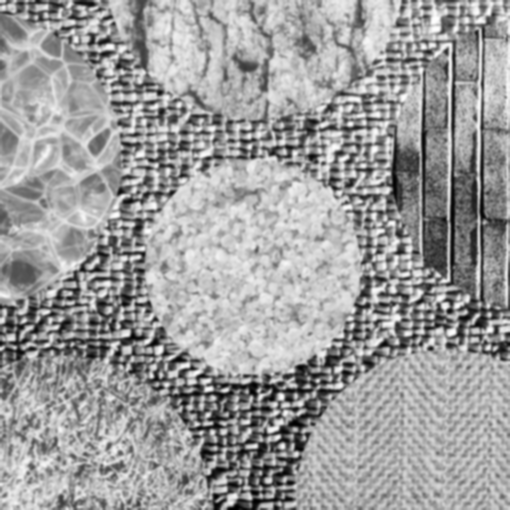
\includegraphics[scale=0.2]{Imagedata_filted_L5L5.png}   
	}
		\qquad
	\subfloat[L5E5 Filter Result] 
	{
		\centering      
		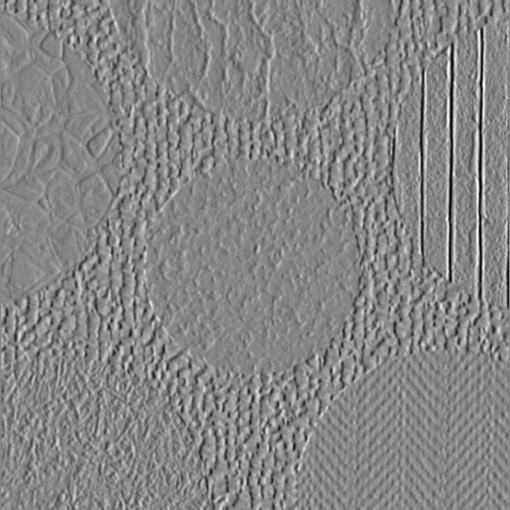
\includegraphics[scale=0.2]{Imagedata_filted_L5E5.png}   
	}
	 \qquad
	\subfloat[L5R5 Filter Result] 
	{
		\centering      
		
\includegraphics[scale=0.2]{Imagedata_filted_L5R5.png}   
	}
	 \qquad
	\subfloat[L5S5 Filter Result] 
	{
		\centering      
		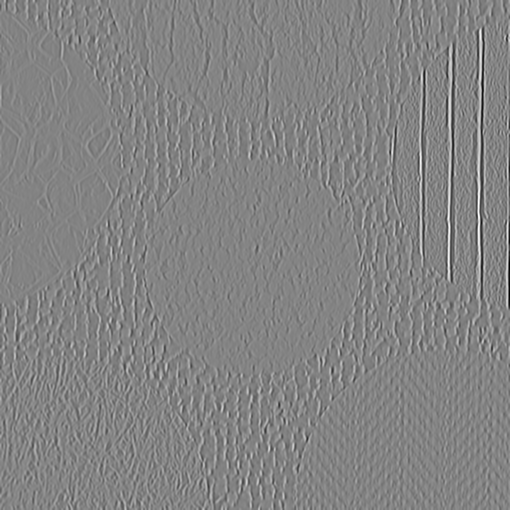
\includegraphics[scale=0.2]{Imagedata_filted_L5S5.png}   
	}
	 \qquad
	\subfloat[L5W5 Filter Result] 
	{
	%	\centering      
		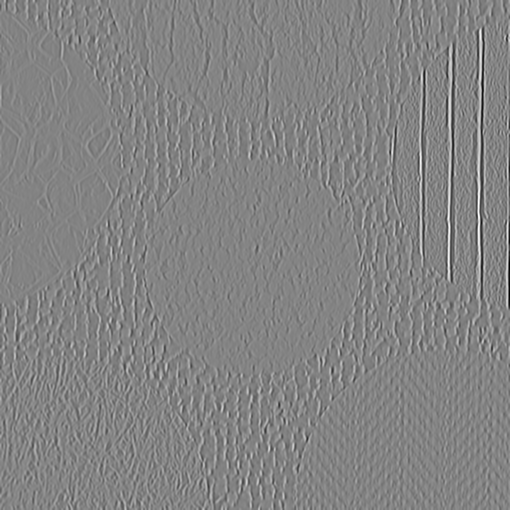
\includegraphics[scale=0.2]{Imagedata_filted_L5W5.png}   
	}
	 \qquad
	\subfloat[E5L5 Filter Result] 
	{
	%	\centering      
		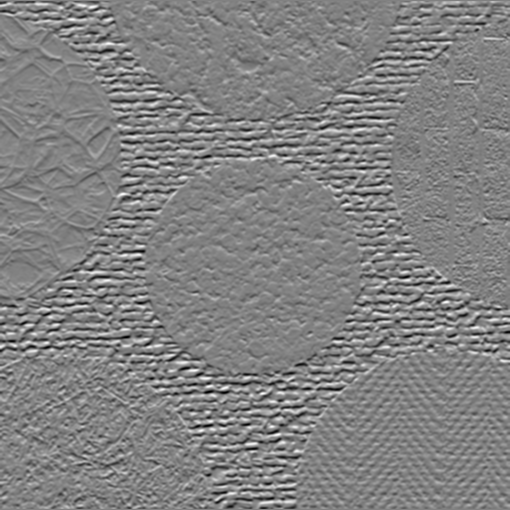
\includegraphics[scale=0.2]{Imagedata_filted_E5L5.png}   
	}
	 \qquad
	\subfloat[E5E5 Filter Result] 
	{
	%	\centering      
		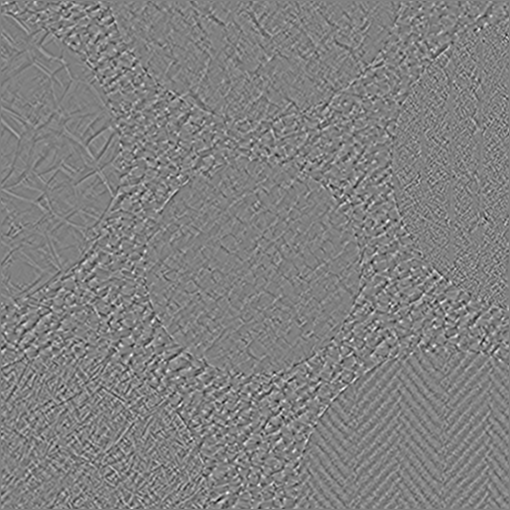
\includegraphics[scale=0.2]{Imagedata_filted_E5E5.png}   
	}
	 
	\caption{Some Filter Result} 
	\label{lawsfiltered}  
\end{figure}

	
	
\item Compute Energy Map\\
Use the Window to produce 25-d energy map.
\begin{equation}
Square\_ sum=\sqrt { \frac { 1 }{ M^2 } \sum _{ i=1 }^{ i=M }{ \sum _{ j=1 }^{ j=M }{ { I(i,j) }^{ 2 } }  }  } 
\end{equation}
Where, M is the window size. Here, I choose $M = 7,15$. Use this value to represent the energy of the pixel located at the center of the window.
\item K-means cluster \\
Apply k-means cluster with 25-D feature space. Set the number of cluster equals to 7. Output the result of the segmented regions by using 7 different grayscale intensity.
\end{enumerate} 
\subsubsection{Experimental Result}

The segmentation result is shown in Figure \ref{texture_seg}.

\subsubsection{Discussion}

Figure \ref{texture_seg} shows the segmentation result is not quite good. There remains some holes in the image and the texture are not clearly classified. That might because the 25-D feature are not strong enought to represent the pixel information. Thus, PCA will not help much in this case.


\subsection{Advanced Texture Segmentation Techniques}
\subsubsection{Abstract and Motivation}
The result of 1(b) is not so clean and in this section I will come up with several idea to enhance the results.
\subsubsection{Approach and Procedures}
\begin{enumerate}
\item Adopt PCA \\
Adapt a PCA method, reduce the 25-D feature space to low dimension feature space. Use the low dimension feature space to do the k-means and output the segmentation result.
\item Post-processing \\
Adapt median filter to merge the small hole and make the segmentation result more cleaning.  The main idea of the median filter is to run through the signal entry by entry, replacing each entry with the median of neighbouthood entries. The pattern of neighbors is called the ``window", which slides, entry by entry, over the entire signal. For 2D images, the window size normally has an odd number of entries, like 3, 5 or 7. Here I choose the window size equal to 21. 

\end{enumerate} 

	
\subsubsection{Discussion}

As I mentioned above, the PCA method does not help much in improving the segmentation result. However, when taking a close look at the detail, {\bf PCA merge some small holes in to a continuous area}.
Although the segmentation result is not so good, but the median filter actually work well in merge the small hole in a specific area. From the Figure \ref{enhance_seg_medfilt2}, we can see that the boundary is more clearly. The k-means method works well in classify the texture located at the right-down area and the middle area.
	


\section{Problem 2: Image Feature Extractor}
\subsection{SIFT}
\subsubsection{Abstract and Motivation}
Scale-invariant feature transform (SIFT) is a computer vision algorithm used to detect and describe local features in image. It looks for the points that invariant in {\bf translation, scaling and rotation} in spatial scale. This algorithm was published by David Lowe in 1999, and was summarized in 2004. In this section, I will introduce the basic procedure of the SIFT algorithm.
\subsubsection{Approach and Procedures}
The foundamental of the SIFT is as follow. The scaling-invariance and position-invariance is achieved by selecting key location at the maxima and minima of the DoG applied in scale space. This key location are treated as the potential key points. First, the input image is continuously filtered and downsampled by stage Gaussian kernel functions with different $\sigma$ and building an image pyramid. After that, we need to remove the points that are not rotation-invariant. It mainly includes the following key steps.

\begin{enumerate}
\item Feature extraction\\
In order to make the features have {\bf position and scale invariance}, the detection of feature points is done in image scale space. The input image is convolved with Gaussian function through several level. 
\begin{equation}
\begin{aligned}
G(\sigma _{ 1 })&=(2\pi \sigma ^{ 2 }_{ 1 })^{ -1 }e^{ -(x^{ 2 }+y^{ 2 })/2\sigma ^{ 2 }_{ 1 } }\\
G(\sigma _{ 2 })&=(2\pi \sigma ^{ 2 }_{ 2 })^{ -1 }e^{ -(x^{ 2 }+y^{ 2 })/2\sigma ^{ 2 }_{ 2 } }\\
G(\sigma _{ 3 })&=(2\pi \sigma ^{ 2 }_{ 3 })^{ -1 }e^{ -(x^{ 2 }+y^{ 2 })/2\sigma ^{ 2 }_{ 3 } }\\
G(\sigma _{ 4 })&=(2\pi \sigma ^{ 2 }_{ 4 })^{ -1 }e^{ -(x^{ 2 }+y^{ 2 })/2\sigma ^{ 2 }_{ 4 } }\\
G(\sigma _{ 5 })&=(2\pi \sigma ^{ 2 }_{ 5 })^{ -1 }e^{ -(x^{ 2 }+y^{ 2 })/2\sigma ^{ 2 }_{ 5 } }
\end{aligned}
\end{equation}
Where $\sigma_{1}= \sqrt { 2 }, \sigma_{2}= 2 , \sigma_{3}= 2\sqrt { 2 }, \sigma_{4}= 4, \sigma_{5}= 4\sqrt { 2 }$.\par
Sample the image with different size. For each specific size, the image are filtered by Gaussian filters with different $\sigma$.
In order to detect stable and unique key points {\bf more efficiently}, then subtract the adjacent gaussian smooth output image to approximate the Laplacian of Gaussian (LoG) with in the same octave. {\bf The computation of DoG cost less than the Computation of LoG.} Then, for each pixels, we choose the 26 neighbourhood pixels to compare with. If it is the minima or maxima of the neighbourhood, we regard it as a potential key point.\par
\item Feature description\\
After get these potential key points, the gradient direction distribution characteristic of the key point's neighborhood pixels is used to assign a direction to each image descriptors, so that the key point has {\bf rotation invariance}.
\begin{equation}
M_{ ij }=\sqrt { (A_{ i,j }-A_{ i+1,j })^{ 2 }+(A_{ i,j }-A_{ i,j+1 })^{ 2 } } 
\end{equation}
\begin{equation}
R_{ i.j }=\tan ^{ -1 }{ (A_{ i,j }+A_{ i+1,j }, } A_{ i,j+1 }+A_{ i,j })
\end{equation}
The pixel differences are efficient to compute and provide sufficient accuracy due to the substantial level of previous smoothing.

\item Removing \\
By removing the potential points that not prossess the rotation-invariance, the key point achieves its robustness of rotation-invariant.
\begin{enumerate}
\item Detect ``Low contrast point" \\
Use Taylor expension method to compute the contrast.
Compute the Hessian matrix $\mtx H$ and its trace and determination.
\begin{equation}
\mtx H=\begin{bmatrix} \mtx D_{ xx } &\mtx D_{ xy } \\\mtx D_{ xy } &\mtx D_{ yy } \end{bmatrix}
\end{equation}
\begin{equation}
tr(\mtx H)=2 \mtx D_{ xy }
\end{equation}
\begin{equation}
det(\mtx H)=\mtx D_{ xy }^2-\mtx D_{ xx }\mtx D_{ yy }
\end{equation}
if 
\begin{equation}
\frac { tr(\mtx H)^2 }{ det(\mtx H) } > \frac { (r+1)^2 }{ r }
\end{equation}
remove it.

\item Remove points in non-salient region\\
In order to make it as stable as possible, the orientation is determined by the peak in the histogram of local imgae gradient orientation. The orientation histogram has 36 bins covering 360 degree range of orientation, ans select the peak value to represent the orientation of the key point.
\end{enumerate} 

\item Illuminance Change\\
SIFT algorithm guarantee its robustness to illuminance change by thresholding the gradient magnitudes with maximum possible gradient value times 0.1. 


\item Output \\
SIFT’s output vector size in its original paper contains 160 elements.
\end{enumerate} 


%\subsubsection{Experimental Result}
%\subsubsection{Discussion}





\subsection{Image Matching}

\subsubsection{Approach and Procedures}
\begin{enumerate}
\item Find the Key-point \& Extract SIFT Feature \\
Input the image {\it river1.raw} and {\it river2.raw} and extract the SIFT feature of the two images. The number of key points found by OpenCV\_SIFT is shown in Figure \ref{numofkey}. The feature extract by OpenCV\_SIFT contains 128 dimensions. 
\begin{figure}[!htp]
	\centering
	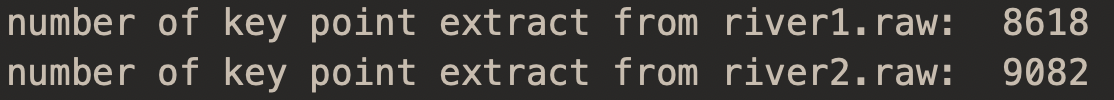
\includegraphics[scale=0.4]{numofkey.png}
	\caption{number of key point found by OpenCV\_SIFT}
	\label{numofkey}
	\end{figure}
\item Find the Largest Scale Key-point\\
The ``largest scale key point" is defined by the key point's corresponding descriptor with the largest $L2$ norm. Thus, by traversing the entire SIFT descriptors of the {\it river1.raw} and caculating the $L2$ norm, I found the largest scale key point $\vct {kp}_1$. The parameters of $\vct {kp}_1$ is shown in Figure \ref{largestscalekp}. The position of $\vct {kp}_1$ is marked in Figure \ref{river1_largest}.


\item Find the Closest Neighboring Key-point
Use K-NN method and compute the $L2$ norm of the distance between $\vct {kp}_1$ and the key-points found in {\it river2.raw}. The $L2$ norm is defined by 
\begin{equation}
\left\| \vct {kp}_{ 1 }-\vct {kp}^{ ' } \right\|_{2} =\sqrt { (x_{ 1 }-{ x }_{ 1 }^{ ' })^{ 2 } + (x_{ 2 }-{ x }_{ 2 }^{ ' })^{ 2 } +...+(x_{ D }-{ x }_{ D }^{ ' })^{ 2 }}
\end{equation}
Where $\vct {kp}^{ ' }$ is the key-point of {\it river2.raw}. the $x_1,x_2...x_D$ are $D = 128$ features of the descriptor, i.e. the 128 entries in a row of the descriptor.
The key-point with the shortest $L2$ norm distance is regardest as the closest neighboring key-point of $\vct {kp}_1$. 
I try several number of nearest neighbour and the result are show in the next section.

\end{enumerate} 
\subsubsection{Experimental Result}
The Nearest Neighbour in {\it river1.raw} and it's orientation is circled in Figure \ref{1nn_river2}. The parameter of the key-point is shown in Figure \ref{1nnpara}

	
\subsubsection{Discussion}

The dominant orientation of the nearest point in {\it river2.raw} is 129.87, which is different from the $\vct {kp}^{ ' }$. Though it is true that in descriptor feature the dominant orientation is provided, this is not used to actually compare the similarity of the keypoints. The keypoints are primarily compared using the distance between the discriptor, which regardless of this dominant orientation are inherently orientation invariant. The dominant orientation are used in some retrieval/classification tasks as extra information used to improve matching scores.


\subsection{Bag of Words}
\subsubsection{Abstract and Motivation}
A Bag-of-Words model that encodes in graphs the local structures of a digital object. In this section, I use the samples of zeros and ones from MNIST to form a codebook with bin size of 2. Use the SIFT algorithm to extract the feature from the image and do k-means cluster. Then, do the classification for the {\it eight.raw} and show the histogram.

\subsubsection{Approach and Procedures}
\begin{enumerate}
\item Extract the SIFT feature\\
Extrac the SIFT feature for each image {\it one\_1.raw} ... {\it zero\_5.raw}. Collect the descriptor for all the image and form a training data set. The OpenCV\_SIFT find 54 key point in total. Thus, the training dataset is a $54 \times 128$ 2-D array.

\begin{figure}[!htp]
	\centering
	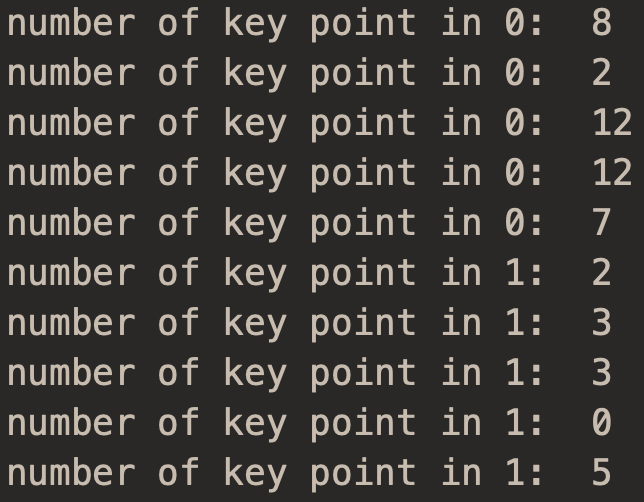
\includegraphics[scale=0.4]{trainset.png}
	\caption{number of key-points}
	\end{figure}
\item K-menas Cluster\\
Train the training set with k-means cluster method and divide the training point into 2 clusters. The zeros' key points are shown in Figure \ref{Zeros} while the ones' key-points are shown in Figure \ref{ones}. The blue dot represent the cluster of object, while the magenta dot reprent the cluster of background.



Finally we got 2 centroid and 2 cluster for futher prediction.
\item Get the Histogram \\
With the trained codebook, I can use it to get the histogram of the {\it eight.raw}. Extract the key-points of {\it eight.raw} and use the discriptor as the prediction dataset. Use the trained k-means cluster above to predict the cluster of the key-points. That is, caculated the $L2$ norm distance between the key-points and two centroids. Label the key-points with the shortest $L2$ norm distance of the centroid.

\item Caculate the Distance

Regarding the histogram as a 2-dimension vector, caculate the distance between $eight.raw$ and the codebook image. First, normalize the vector so that it has unit length. Then caculate the $L2$ norm of the distance and take an average. Use this distance information to classify the target image.
 
\end{enumerate} 

	
	
\subsubsection{Discussion}

From the Table \ref{dist}, we can result that the {\it eight.raw} is closer to image zeros than ones. If there is only two digits in the bag, then {\it eight.raw} will be classified as Zeros.

The OpenCV\_SIFT detect 12 points in {\it eight.raw}, however, only 5 of them are marked in the Figure \ref{eight_kp}. The reason is that some key-points {\bf share the same coordinate but different in angle}. 


%\section{Problem 1: Texture Analysis}
%\subsection{Texture Classification}
%\subsubsection{Abstract and Motivation}
%\subsubsection{Approach and Procedures}
%\subsubsection{Experimental Result}
%\subsubsection{Discussion}

%\begin{figure}[!htp]
%	\centering
%	\includegraphics[scale=0.3]{cat.eps}
%	\caption{cat.raw}
%	\end{figure}


%\begin{enumerate}
%\item good morning...
%\item good morning....
%\end{enumerate} 
%
%
%
\end{document}

